% Chapter 03
% !TEX encoding = UTF-8 Unicode
\chapter{Parent of origin gene expression in a founder population identifies two novel imprinted genes at known imprinted regions.}\label{ch:imprinted}
\section[Abstract]{Abstract\footnotemark}


Genomic imprinting is the phenomena that leads to silencing of one copy of a gene inherited from a specific parent. Mutations in imprinted regions have been involved in diseases showing parent of origin effects, such as Prader-Willi and Angelman syndrome, among others. Identifying genes with evidence of parent of origin expression patterns in family studies allows the detection of more subtle imprinting. Here we use allele specific expression in lymphoblastoid cell lines from 306 Hutterites related in a single pedigree to provide formal evidence for parent of origin effects. Our approach identified known imprinted genes, two putative novel imprinted genes, and 14 genes with asymmetrical parent of origin gene expression. We used gene expression in peripheral blood leukocytes (PBL) to validate our findings, and then confirmed imprinting control regions (ICRs) using DNA methylation levels in the PBLs.


\footnotetext{Citation for chapter: Mozaffari SV, Stein MM, Magnaye KM, Nicolae DL, Ober C. Gene Expression and Methylation of Imprinted Genes in the Hutterites bioRxiv (2018).}

\section{Introduction}\label{ch03-introduction}
	Imprinted genes have one allele silenced in a parent of origin specific manner. In humans, approximately 105 imprinted loci have been identified, many of which play important roles in development and growth \cite{Falls1999,Peters2014}. Dysregulation of imprinted genes or regions can cause diseases that show parent of origin effects, such as Prader-Willi or Angelman syndrome, among others \cite{Peters2014}. Imprinted regions have also been associated with complex traits, such as height and age of menarche \cite{Benonisdottir:2016dz,Zoledziewska:2015do}, as well as common diseases such as obesity and some cancers \cite{Peters2014}. More than 80\% of imprinted genes in humans are clustered in genomic regions that contain both maternally and paternally expressed genes, as well as genes that encode non-coding RNAs. Parent-specific expression of the genes within a cluster are maintained by complex epigenetic mechanisms at cis-acting imprinting control regions (ICRs) \cite{Kalish:2014gd}, which show parent of origin specific DNA methylation patterns and chromatin modifications.
	
Using RNA-seq and allele specific expression (ASE) we can map genes to parental haplotypes and identify those that are expressed when inherited from only the father or only from the mother, a hallmark feature of imprinted loci. Parent of origin effects and imprinted genes have been most elegantly studied in mice, where two inbred strains are bred reciprocally to identify parent of origin effects on gene expression in progeny that have the same genotypes but different patterns of inheritance \cite{Babak2015}. Additionally, uniparental inheritance of imprinted regions in mice were associated with abnormal developmental phenotypes\cite{Cattanach:1985hu} before it was shown that imprinting defects are associated with human disease \cite{Nicholls:vh}. One approach to identifying imprinted loci in humans has been to test for parent of origin effects on gene expression and phenotypes in pedigrees \cite{Kong:2009kk,Benonisdottir:2016dz}. For example, Garg et al. used gene expression in LCLs from HapMap trios to identify 30 imprinting eQTLs with parent of origin specific effects on expression including two imprinted genes \cite{Garg2012a}. A study from the GTEx Consortium used RNA-seq data and allele specific expression to identify allelic imbalance in 45 different tissues. By considering genes with monoallelic expression that was evenly distributed to both the reference and alternate alleles across individuals as evidence for imprinting, they identified 42 imprinted genes, both known and novel, and used family studies to confirm imprinting of 5 novel imprinted genes \cite{Baran:2015cx}. Santoni et al. identified nine novel imprinted genes using single-cell allele-specific gene expression and identifying genes with mono-allelic expression in fibroblasts from 3 unrelated individuals and probands of 2 family trios, and then using the trios to confirm parent of origin of the alleles \cite{Santoni:2017hu}.

Here, we perform a parent of origin ASE study in a large pedigree to characterize parent of origin specific gene expression in the Hutterites, a founder population of European descent, for which we have phased genotype data \cite{Livne2015}. We use RNA-seq from lymphoblastoid cell lines (LCLs) to map transcripts to parental haplotypes and identify known and two not previously reported imprinted genes. We validated the two putative imprinted genes by showing the same patterns of parent of origin expression PBLs from different Hutterite individuals, and show DNA methylation signatures of imprinting in the PBLs at these regions.
	
\section{Results}\label{ch03-results}
\subsection{Mapping Transcripts to Parental Haplotypes}\label{Mapping Transcripts to Parental Haplotypes}
For each of 306 individuals, the total number of transcripts at each gene was assigned as maternally inherited, paternally inherited, or unknown parent of origin. The last group included transcripts without heterozygote SNPs or SNPs without parent of origin information. Transcripts were assigned to the parentally inherited categories using SNPs in the reads and matching alleles to either the known maternally or paternally inherited alleles. All the genes analyzed had some transcripts of unknown origin (average 97.8\%, range 8.3-100\%). For each gene we assigned parental origin to an average of 1.8\% of transcripts (range: 0-34.7\%), and for each individual we assigned parental origin to an average of 1.4\% of transcripts (range: 0-1.7\%). On average, about 40 SNPs per gene were used to assign the transcripts of a gene to parent (range 1-1839 SNPs). 



\begin{table}
\centering
\begin{adjustbox}{width={\textwidth}}
\begin{tabular}{@{}p{10cm}p{2cm}p{4cm}p{2cm}@{}}
\toprule & Mean & Standard Deviation & Range \\ \midrule
 Proportion of transcripts from each gene assigned to transcripts of unknown origin & 0.978 & 0.031 & (0.083, 1) \\
 Proportion of transcripts from each gene assigned to parental origin & 0.018 & 0.019 & (0, 0.347) \\
 Proportion of transcripts for each individual assigned to parental origin & 0.014 & 0.0015 & (0, 0.017) \\ \bottomrule
\end{tabular}
\end{adjustbox}
\caption[Summary Statistics for Parental Origin of Transcripts.]{\textbf{Summary Statistics for Parental Origin of Transcripts.}}
\label{tab:summarystats}
\end{table}




After quality control (see Methods), transcripts in 15,889 genes were detected as expressed in 306 individuals. Some transcripts for 14,791 of those genes could be assigned to a parent. Of these, 75 genes were only expressed on the paternally-inherited allele in at least one individual and not on the maternally inherited allele in any individuals. Similarly, 64 genes were only expressed on the maternally-inherited allele in at least one individual and not on the paternally inherited allele in any individuals (S1 Table).

\subsection{Imprinted Genes in Lymphoblastoid Cell Lines (LCLs)}\label{Imprinted Genes in Lymphoblastoid Cell Lines (LCLs)}
Among the 139 genes with only paternally inherited expression or only maternally inherited expression, there are three known imprinted genes (\emph{CDKN1C}, \emph{NDN}, \emph{SNRPN}) and one predicted to be imprinted (\emph{IFITM1}) \cite{Luedi:2007ib}. \emph{CDKN1C} showed patterns opposite of what has been reported\cite{Hatada:1995jf,Matsuoka:1996uq}, which could be due to the small sample (only three individuals showed expression from one parent) or to the different cell types used here (LCLs) and in previous studies (developing brain and embryonal tumors for CDKN1C).

We expect some imprinted genes to have ``leaky" expression, such that there is some expression from the parental chromosome that is mostly silenced. To detect these genes, we used a binomial test to find patterns of gene expression asymmetry by parental transcript levels.  This analysis identified 28 genes with an FDR \textless5\% (Table \ref{tab:imprintedgenes}). The 11 genes that showed the most asymmetry are known imprinted genes: \emph{ZDBF2}, \emph{PEG10}, \emph{SNHG14}, \emph{NHP2L1}, \emph{L3MBTL1}, \emph{ZNF331}, \emph{LPAR6}, \emph{FAM50B}, \emph{KCNQ1}, \emph{NAP1L5}, and \emph{IGF1R}. Parent of origin expression for \emph{ZDBF2} and \emph{KCNQ1} are shown in Fig \ref{fig:matpatexpression}A and \ref{fig:matpatexpression}B, respectively. We identified two additional genes that showed asymmetry in parental expression from mostly one parent (\emph{PXDC1}, \emph{PWAR6}), which we consider potentially new imprinted genes. The remaining fourteen genes showed significant patterns of asymmetry but had expression from both maternal and paternal transcript levels. These genes are likely not imprinted but could have asymmetry in expression due to an expression quantitative trait loci (eQTL). 



\begin{table}
\centering
\begin{adjustbox}{width={\textwidth}}
\begin{tabular}{@{}p{3cm}|p{2cm}p{5cm}p{5cm}p{6cm}@{}}
\toprule Gene & p-value & Number of individuals with more maternal expression than paternal expression & Number of individuals with more paternal expression than maternal expression & References \\ \midrule
 \multicolumn{5}{c}{A. Known Imprinted}  \\ \hline
 \emph{ZDBF2} & 1.59e-41 & 2 & 148 & geneimprint.com, Baran et al\citep{Baran:2015cx}, and Babak et al.\citep{Babak2015} \\
 \emph{PEG10} & 5.51e-38 & 2 & 136 & geneimprint.com, Baran et al\citep{Baran:2015cx}, and Babak et al.\citep{Babak2015} \\
 \emph{SNHG14} & 1.64e-36 & 2 & 131 & Baran et al\citep{Baran:2015cx} \\
 \emph{NHP2L1} & 1.24e-33 & 23 & 189 & Babak et al.\citep{Babak2015}  and Docherty et al. \citep{Docherty:2014cx} \\
 \emph{L3MBTL1} & 6.72e-31 & 2 & 107 & geneimprint.com, and Li et al. \citep{Li:2004km}\\
 \emph{ZNF331} & 4.05e-25 & 36 & 184 & Daelemans et al.\citep{Daelemans:2010kc} and Baran et al\citep{Baran:2015cx} \\
 \emph{LPAR6} & 2.65e-23 & 9 & 76 & Baran et al\citep{Baran:2015cx}\\
 \emph{FAM50B} & 5.29e-23 & 0 & 75 & geneimprint.com, Baran et al\citep{Baran:2015cx}\\
 \emph{KCNQ1} & 1.34e-22 & 79 & 1 & geneimprint.com, Baran et al\citep{Baran:2015cx} \\
 \emph{NAP1L5} & 3.76e-09 & 0 & 29 & geneimprint.com \\
 \emph{IGF1R} & 1.11e-05 & 14 & 49 & geneimprint.com, Sun et al. \citep{Sun:2014eq}, Kang et al. \citep{Kang:2015ko}, Boucher et al. \citep{Boucher:2014gk}, and Al Adhami et al.\citep{AlAdhami:2015dx}\\
 \multicolumn{5}{c}{B. Conflicting Evidence for Imprinting Status in the Literature}  \\ \hline
\emph{PRIM2} & 5.53e-05 & 30 & 71 & geneimprint.com, Santoni et al. \citep{Santoni:2017hu}\\
\multicolumn{5}{c}{C. New Imprinted Genes}  \\ \hline
 \emph{PXDC1} & 9.83e-14 & 12 & 81 & - \\
 \emph{PWAR6} & 2.27e-13 & 0 & 43 & - \\
 \multicolumn{5}{c}{D. Genes with Asymmetrical Parent of Origin Expression}  \\ \hline
 \emph{SNHG17} & 6.2e-08 & 113 & 45 & - \\
 \emph{ZNF813} & 8.7e07 & 63 & 132 & - \\
 \emph{DAAM1} & 1.78e-05 & 66 & 126 & -\\
 \emph{RP11-379H18.1} & 2.09e-05 & 52 & 106 & - \\
 \emph{HMGN1P38} & 2.09e-05 & 52 & 106 & - \\
 \emph{MTX2} & 3.05-05 & 0 & 16 & - \\
\emph{ZNF714} & 4.61e-05 & 35 & 79 & - \\
\emph{MAF1} & 4.45e-05 & 17 & 51 & - \\
\emph{IL16} & 5.71e-05 & 61 & 115 & - \\
\emph{CPNE1} & 5.56e-05 & 111 & 58 & - \\
\emph{ATP6V0D1} & 7.03e-05 & 32 & 7  & - \\
\emph{FAHD1} & 9.34e-05 & 68 & 29 & - \\
\emph{CNN2} & 1.18e-04 & 127 & 72 & -\\
\emph{HSP90AB3P} & 1.16e-04 & 7 & 31 & - \\ \bottomrule
\end{tabular}
\end{adjustbox}
\caption[Results for Genes with Parent of Origin Expression Asymmetry. ]{\textbf{Results for Genes with Parent of Origin Expression Asymmetry. }
Genes listed by category of imprinting status: (A) Known Imprinted, (B) Conflicting Evidence for Imprinted Status, (C) New Imprinted Genes, (D) Genes with Asymmetrical Parent of Origin Expression. Genes are ordered by significance within each category.}
\label{tab:imprintedgenes}
\end{table}




\begin{figure}[!htb]
\centering 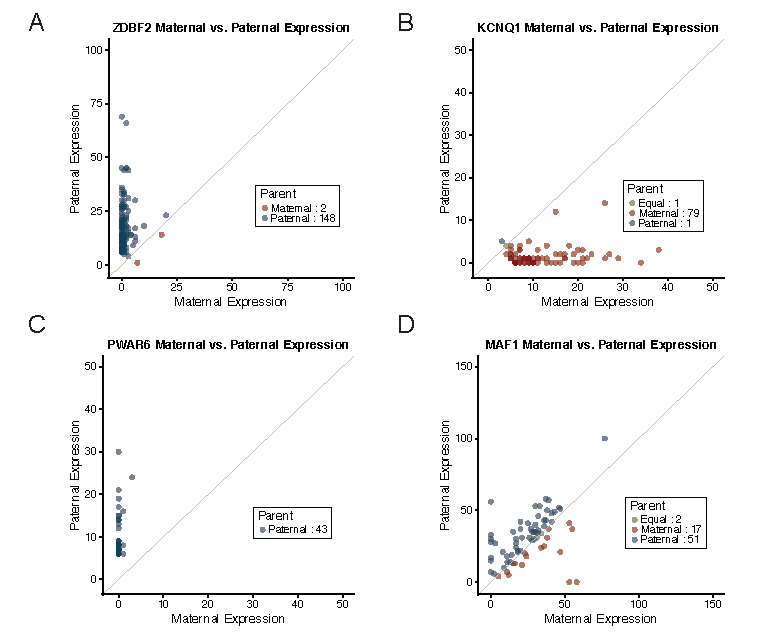
\includegraphics[width=7in]{img/ch03/fig-01.pdf}
\caption[Plot of maternal (x-axis) and paternal (y-axis) gene expression for four genes.]{\textbf{Plot of maternal (x-axis) and paternal (y-axis) gene expression for four genes.} Plot of maternal (x-axis) and paternal (y-axis) gene expression for four genes. (A) maternally imprinted gene \emph{ZDBF2} (paternally expressed), (B) paternally imprinted gene \emph{KCNQ1} (maternally expressed), (C) novel maternally imprinted gene \emph{PWAR6} (paternally expressed), (D) gene with asymmetry in parental expression \emph{MAF1}. Each point represents one individual. Numbers in the legend represent the number of individuals with equal maternal and paternal expression, more maternal expression, or more paternal expression.}
\label{fig:matpatexpression}
\end{figure}


Two genes showed gene expression signatures consistent with imprinting but have not previously been recognized as imprinted genes. The first potentially new imprinted gene is \emph{PXDC1}, which is in the same region and next to (\textless100kb) a known imprinted gene, \emph{FAM50B}. The second potentially novel imprinted gene is \emph{PWAR6}, or Prader Willi Angelman Region RNA6, a gene encoding regulatory class of RNA. Although this gene is located within the intron of a known imprinted region, \emph{SNHG14}, this noncoding RNA has not previously been recognized as having parent of origin specific expression (Fig 1C).

The remaining fourteen genes show significant asymmetry using the binomial test but do not have expression from mostly one parental chromosome. One of these genes, \emph{SNHG17}, is a noncoding RNA. Another gene with parent of origin asymmetry,  \emph{ZNF813}, is next to a known imprinted gene, \emph{ZNF331}. The remaining genes with asymmetrical parent origin expression have expression from both parental chromosomes, unlike imprinted genes. These genes include  \emph{DAAM1},  which is involved in cytoskeleton, specifically filopodia formation \citep{Hoffmann:2014ki, Luo:2016db}, and has a suggested role for cytoskeleton organization during Mammalian testis morphogenesis and gamete progression \citep{Pariante:2016kn};  \emph{RP11-379H18.1}, a noncoding RNA gene;  \emph{HMGN1P38} \citep{StrichmanAlmashanu:2003cw}; MTX2, a nuclear gene that interacts with mitochondrial membrane protein metaxin 1 and is involved in mitochondrial protein import and metabolism of proteins in mice;   \emph{MAF1} a negative regulator of RNA polymerase 2;  \emph{ZNF714},  \emph{CPNE1},  \emph{IL16},  \emph{ATP6V0D1},  \emph{FAHD1},  \emph{HSP90AB3P}, and  \emph{CNN2} are the remaining genes that show parent of origin asymmetry but not with a pattern consistent with imprinting (S1 Figure).

\subsection{Validation of Imprinted Genes in PBLs}\label{Validation of Imprinted Genes in PBLs}
Using the same methods described above, we assigned parent of origin to transcripts in PBLs from 99 Hutterite individuals not included in the LCL studies. Maternal and paternal expression in PBLs for all 28 genes identified in LCLs showed similar trends of asymmetry as in LCLs (Figure \ref{fig:matpatPBLs}). 


\begin{figure}[!htb]
\centering 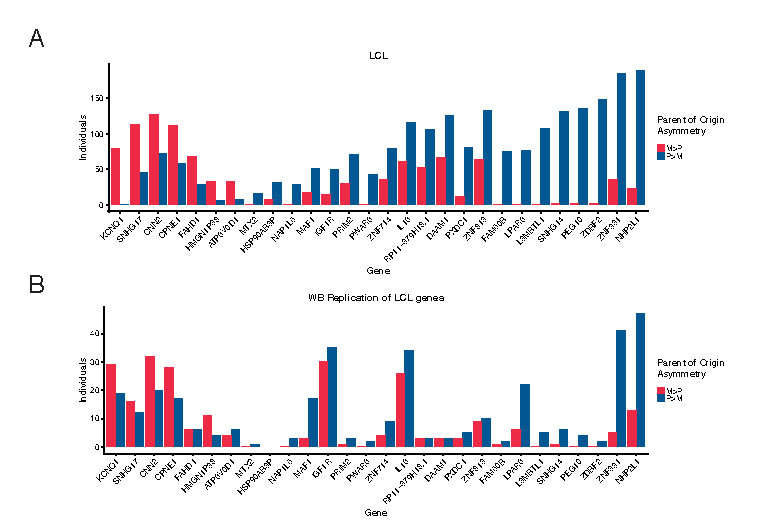
\includegraphics[width=6in]{img/ch03/fig-02.pdf}
\caption[Validation in PBLs.]{\textbf{Validation in PBLs.}Histogram showing the number of individuals with more maternal expression (M \textgreater P) or more paternal expression (P \textgreater M) for the 28 genes showing parent of origin asymmetry in LCLs (A) and PBLs (B) Genes are ordered by the magnitude of the difference in the number of individuals with more maternal expression than paternal expression in LCLs. }
\label{fig:matpatPBLs}
\end{figure}


\subsection{Methylation at Imprinting Control Regions}\label{Methylation at Imprinting Control Regions}
One of the mechanisms underlying parent of origin effects on expression at imprinted loci is differential methylation at cis-acting imprinting control regions (ICRs). DNA methylation from the Illumina HumanMethylation 450K array was available in PBLs from the same individuals included in the validation studies described above. To determine the expected patterns of methylation at known imprinted loci, we first looked at previously characterized methylated regions at known imprinted regions from Court et al. and Joshi et al. \cite{Court:2014kc,Joshi:2016bb}.

The methylation patterns at the two potentially novel imprinted genes identified in this study, \emph{PXDC1} and \emph{PWAR6}, lie in or near known imprinted regions that contain previously characterized ICRs. These previously characterized ICRs show about 50\% methylation (beta value of between 0.25 and 0.75) in our DNA methylation data, which likely reflect methylation at only one parental chromosome in all the cells in the sample. Methylation patterns in PBLs at these two ICRs fall within this hemi-methylation range, further suggesting that these two genes are indeed imprinted (Fig \ref{fig:methylation}).


\begin{figure}[!htb]
\centering 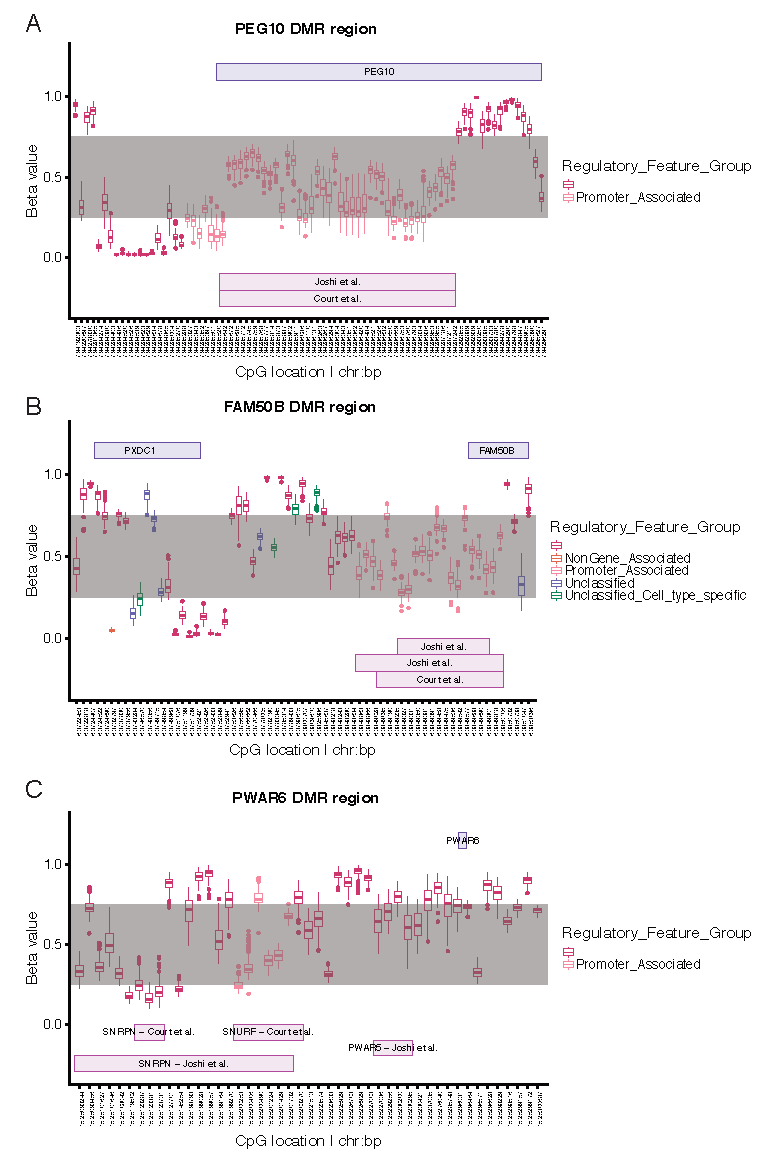
\includegraphics[width=5in]{img/ch03/fig-03.pdf}
\caption[Methylation at ICRs.]{\textbf{Methylation at ICRs.} DNA methylation levels near known and novel imprinted genes previously defined by Joshi et al. and Court et al. (A) \emph{PEG10}, (B) \emph{PXDC1} and \emph{FAM50B}, (C) \emph{PWAR6}.}
\label{fig:methylation}
\end{figure}


\section{Discussion}\label{ch03-discussion}
Dysregulation of imprinted genes can have a large impact on mammalian development and has been associated with significant diseases in humans. Studies aimed at identifying imprinted genes at genome-wide levels have used allele specific expression and imbalance to infer parent of origin. Here we used a large pedigree with assigned parent of origin alleles to map transcripts to chromosomes with known parent of origin and identify imprinted genes. 

Using this approach, we found genes with expression primarily from either the maternal or paternal haplotype. Because gene silencing at imprinted loci may be incomplete, we used a binomial test on parent of origin gene expression and identified 11 known imprinted genes and two potentially novel imprinted genes. Both of these novel genes, \emph{PWAR6} and \emph{PXDC1}, lie in known imprinted regions but have not themselves been characterized as imprinted. The remaining genes that have significant parent of origin asymmetry in gene expression do not show clear imprinting expression patterns. To validate these findings, we mapped gene expression in PBLs from Hutterite individuals not included in the LCL study. The same genes showed similar patterns of asymmetry in these different cell sources (transformed B cells and peripheral blood leukocytes) from different individuals.

In addition to validating gene expression, we characterized methylation patterns near genes showing asymmetry. Using results from studies that had previously characterized ICRs in patients with uniparental disomy at many imprinted regions \citep{Joshi:2016bb, Court:2014kc}, we estimated regions for defining hemi-methylation near the genes identified in our study. Using this approach, we were able to provide additional supportive data for the two potentially novel imprinted genes to be true imprinted genes regulated by previously characterized ICRs. 

Although our study is the largest pedigree-based study to date to search genome-wide for imprinted genes, it has limitations. First, we are able to determine the parent of origin for many transcripts in the Hutterites but we could not assign every RNA sequencing read to a parent due to lack of heterozygous sites or missing parent of origin information for alleles. Second, we conducted these studies in lymphoblastoid cell lines, and therefore could only study genes imprinted in this cell type and would miss the many imprinted genes that are tissue-specific and/or developmentally regulated. Third, while we can verify previously characterized ICRs, our study is not designed to identify novel ICRs because DNA methylation values from an array cannot be assigned to parental haplotype. Lastly, although we characterized the gene expression and methylation patterns for two potentially novel imprinted genes, replication of these genes in a different population and in different tissues, and functional characterization of these genes are required to confirm their status as imprinted genes. Similarly, some of the other genes with parent of origin asymmetry in the blood cells examined in this study may show more clear-cut evidence for imprinting in other tissues or at specific periods of development.  

In summary, we have identified two new imprinted genes using gene expression from a founder population. The genes with asymmetrical parental expression had similar patterns of asymmetry in a different source of blood cells and in different individuals, and we were able to replicate the methylation patterns in known ICRs near the known and novel imprinted genes in this study. Our method and study population allowed us to map reads to parental haplotypes and uncovered \emph{PWAR6} and \emph{PXDC1} as new imprinted genes that could potentially impact disease risk and development.

\section{Methods}\label{ch03-methods}

\subsection{Genotypes}\label{Genotypes}
Hutterite individuals (n=1,653) were genotyped using one of three Affymetrix genotype arrays, as previously described\citep{Livne2015}, of which 121 underwent whole genome sequencing by Complete Genomics, Inc (CGI) (n=98) or Illumina whole genome sequencing (n=27). A total of 10,235,233 variants present in the sequenced individuals were imputed and phased to the remaining 1532 genotyped individuals using PRIMAL \citep{Livne2015}. Parent of origin was assigned to 89.85\% of the alleles with call rate 81.6842\% after QC. For this study, we included individuals with genotyped parents in the primary analyses in LCLs. Written consents for these studies were obtained from the adult participants and parents of children under 18; written assents were obtained from all children. This study was approved by the University of Chicago Institutional Review Board.   

\subsection{RNA-seq in Lymphoblastoid Cell Lines (LCLs).}\label{RNA-seq in Lymphoblastoid Cell Lines (LCLs).}
RNA-seq was performed in LCLs as previously described \citep{Cusanovich:2016id}. For this study, sequencing reads were reprocessed as follows. Reads were trimmed for adaptors using Cutadapt (reads less than 5 bp discarded) then remapped to hg19 using STAR indexed with gencode version 19 gene annotations \citep{Dobin:2002by, Martin:2011eu}. To remove mapping bias, reads were processed and duplicate reads removed using WASP \citep{vandeGeijn:2015hi}. We used a custom script modified from WASP to separate reads that overlap maternal alleles or paternal alleles. Reads without informative SNPs (homozygous, or no parent of origin information) were categorized as unknown where the unknown, maternal, and paternal make up the total gene expression. Gene counts were quantified using STAR for each category. VerifyBamID was used to identify sample swaps \citep{Jun:2012je}. Genes mapping to the X and Y chromosome were removed; genes with a CPM log transformed value less than 1 in less than 20 individuals were also removed.

\subsection{RNA-seq in Peripheral Blood Leukocytes (PBLs) }\label{RNA-seq in Peripheral Blood Leukocytes (PBLs) }
RNA-seq was performed in whole blood as previously described \citep{Stein:2016hn}. For this study, sequencing reads were reprocessed as described above for the studies in LCLs. For all analyses, we excluded 32 individuals who were also in the LCL study.

\subsection{Identifying Imprinted Genes}\label{Identifying Imprinted Genes}
We used a binomial test to detect asymmetry in parent of origin gene expression. We generated a binomial Z-score for each individual for each gene ($Z_i$) and excluded those where $Z_i =0$. For each gene, the number of subjects with $Z_i >0$ can be modeled by a Binomial distribution with probability 1/2. For imprinted genes that show patterns of asymmetry, we expect a distribution of Z-scores that are skewed to one direction: right-skewed for genes asymmetrically maternally expressed and left-skewed for genes asymmetrically paternally expressed. Because we are only asking whether there are more individuals with more maternal expression or more paternal expression and not gene expression measures there is no need to model over-dispersion.

\subsection{DNA methylation profiling and processing in PBLs}\label{DNA methylation profiling and processing in PBLs}
One milliliter of whole blood from 145 Hutterites was drawn into TruCulture (Myriad RBM; Austin, Texas) tubes containing proprietary TruCulture media. DNA was extracted using AllPrep DNA/RNA Mini Kits (Qiagen). DNA samples were bisulfite converted and hybridized to the Illumina HumanMethylation 450K array at the University of Chicago Functional Genomics Center.  Samples were processed using default parameters using the R package minfi \citep{Aryee:2014by}, normalized using SWAN (subset within-array normalization \citep{Maksimovic:2012ib}) and quantile normalized similar to previous methylation studies \citep{NicodemusJohnson:2016go}.  Probes were removed if: (1) mapped non-uniquely to a bisulfite-converted genome; (2) mapped to sex chromosomes; (3) had a probe detection p-value \textgreater0.01 in at least 25\% of samples; and (4) contained common SNPs within the probe sequence, as previously described\citep{Banovich:2014bn}. Principal components analysis (PCA) was used to identify significant technical covariates, and the ComBat function \citep{Johnson:2007fp} within the R package sva \citep{Leek:2012ee} was used to correct for chip effect. Analyses of DNA methylation levels were conducted using beta values, which were converted from M-values using the lumi R package \citep{Du:2008ev}.






\begin{figure}[!htb]
\centering 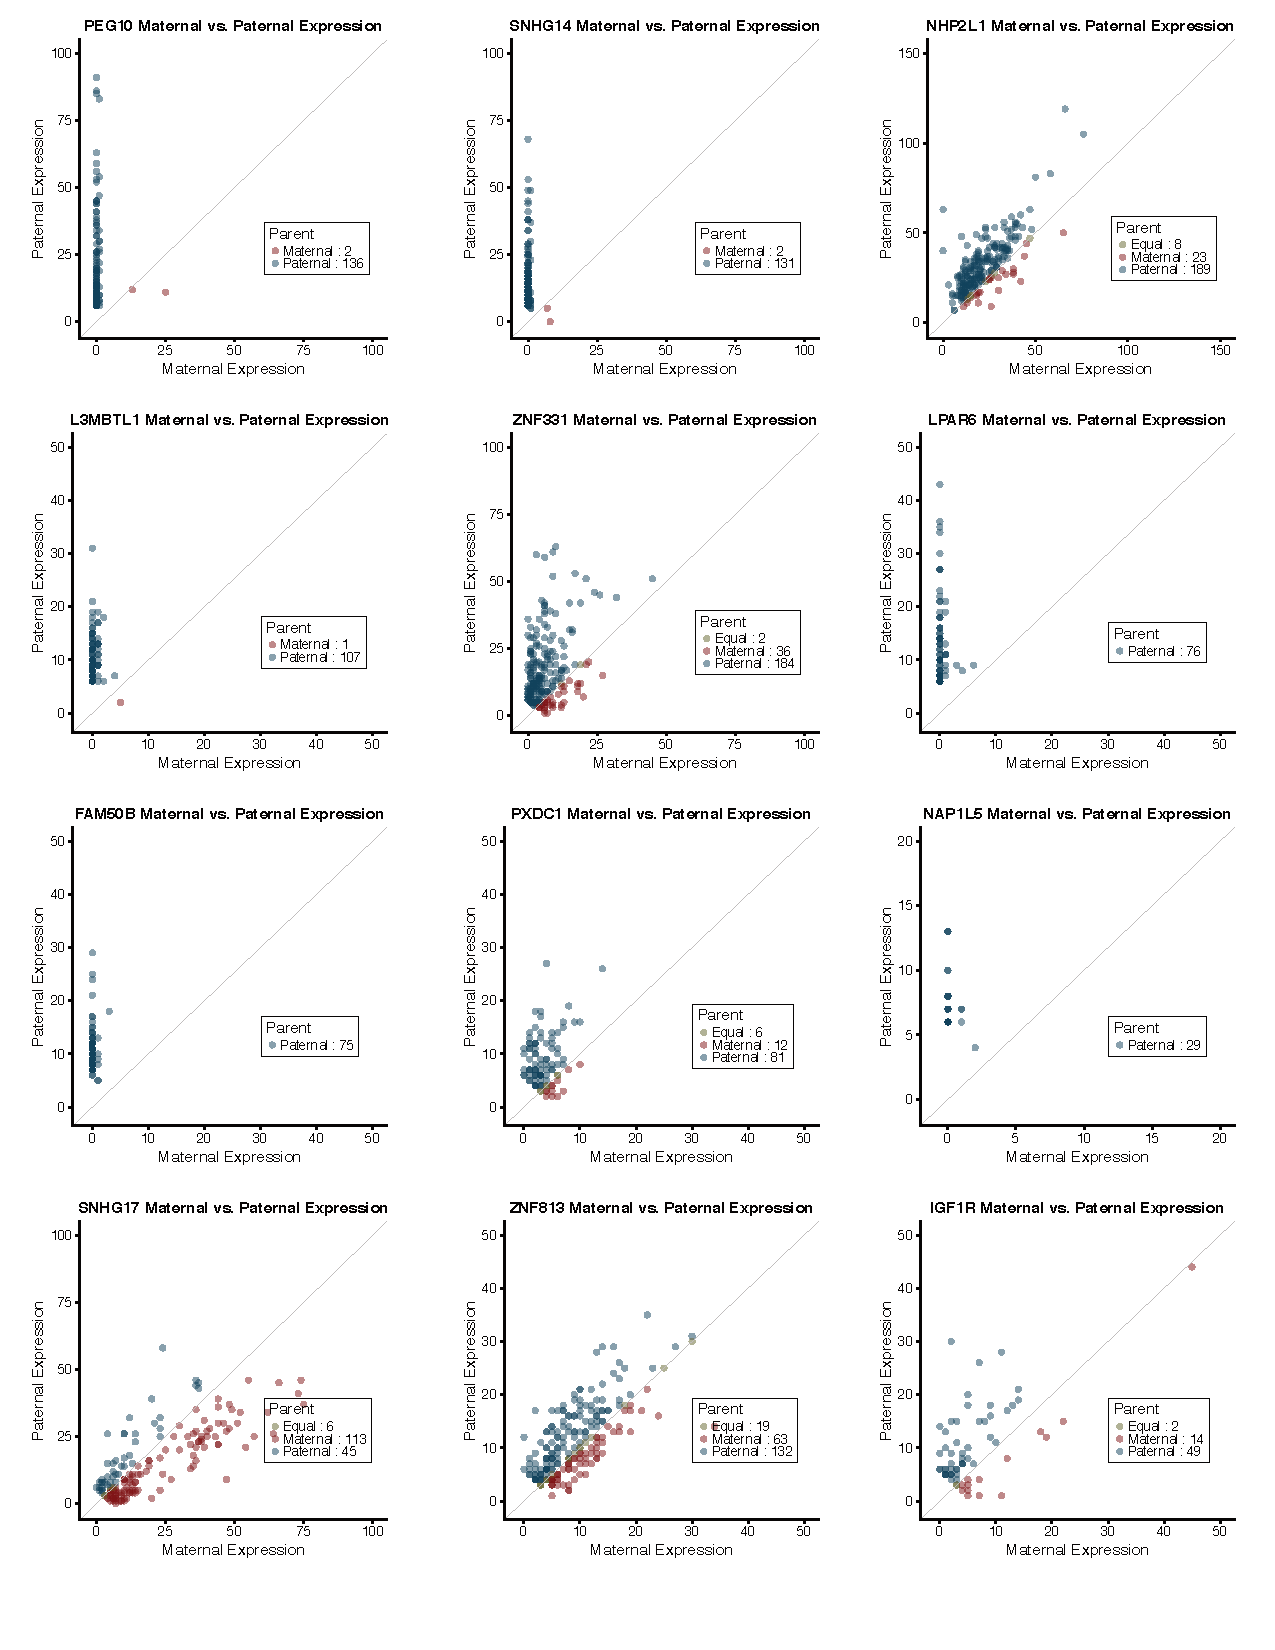
\includegraphics[width=5in]{img/ch03/fig-s1.pdf}
\caption[Plots of maternal and paternal expression for remaining genes with parent of origin asymmetry.]{\textbf{Plots of maternal and paternal expression for remaining genes with parent of origin asymmetry.} Maternal gene expression along x-axis and paternal gene expression along y-axis.}
\label{fig:matpatgexp}
\end{figure}





\begin{figure}[!htb]
\centering 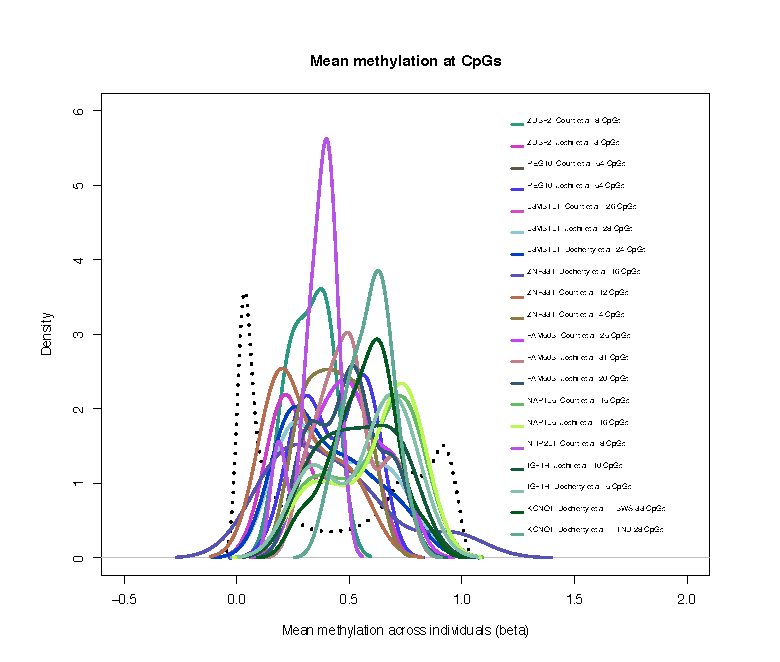
\includegraphics[width=5in]{img/ch03/fig-s2.pdf}
\caption[Density plot for DMRs for all imprinted genes.]{\textbf{Density plot for DMRs for all imprinted genes.} DNA methylation density plots for all imprinted genes with methylation levels in Joshi \emph{et al}\citep{Joshi:2016bb} and Court \emph{et al.}\citep{Court:2014kc} }
\label{fig:methylationdensity}
\end{figure}


%\begin{landscape}
\begin{table}[!htb]
\centering
\begin{adjustbox}{width={\textwidth}}
\begin{tabular}{@{}p{4cm}p{3cm}p{3cm}p{3cm}p{3cm}p{3cm}@{}}
\toprule Gene & 	Number of \newline Individuals & 	Gene Name&	Imprinted \newline Status	&Observed \newline Expression \newline Pattern \newline in LCLs	&Pattern \newline consistent with \newline known \newline expression? \\ \midrule
ENSG00000182636 & 22 & \emph{NDN} & Known & Paternal & Consistent\\ \hline
ENSG00000259261 & 11 & \emph{IGHV4OR15-8} & &  Maternal &   \\ \hline
ENSG00000128739 & 9 & \emph{SNRPN} & Known & Paternal & Consistent\\ \hline
ENSG00000185044 & 9 & \emph{RP11-435B5.4} & &  Maternal &   \\ \hline
ENSG00000089876 & 6 & \emph{DHX32} & &  Paternal &   \\ \hline
ENSG00000262333 & 5 & \emph{HNRNPA1P16} & &  Paternal &   \\ \hline
ENSG00000196378 & 5 & \emph{ZNF34} & &  Maternal &   \\ \hline
ENSG00000198744 & 5 & \emph{RP5-857K21.11} & &  Maternal &   \\ \hline
ENSG00000233757 & 5 & \emph{AC092835.2} & &  Maternal &   \\ \hline
ENSG00000272933 & 5 & \emph{RP11-47A8.5} & &  Maternal &   \\ \hline
ENSG00000154611 & 4 & \emph{PSMA8}& &  Paternal &   \\ \hline
ENSG00000228109 & 4 & \emph{MFI2-AS1} & &  Paternal &   \\ \hline
ENSG00000103269 & 4 & \emph{RHBDL1} & &  Maternal &   \\ \hline
ENSG00000129654 & 4 & \emph{FOXJ1} & &  Maternal &  \\ \hline
ENSG00000129757 & 3 & \emph{CDKN1C} & Known & Paternal & Inconsistent\\ \hline
ENSG00000137936 & 3 & \emph{BCAR3}& &  Paternal &   \\ \hline
ENSG00000148926 & 3 & \emph{ADM} & &  Paternal &   \\ \hline
ENSG00000204482 & 3 & \emph{LST1} & &  Paternal &   \\ \hline
ENSG00000211669 & 3 & \emph{IGLV3-10} & &  Paternal &   \\ \hline
ENSG00000223509 & 3 & \emph{RP11-632K20.7} & &  Paternal &   \\ \hline
ENSG00000260442 & 3 & \emph{RP11-22P6.3} & & Paternal &   \\ \hline
ENSG00000270441 & 3 & \emph{RP11-694I15.7} & &  Paternal &   \\ \hline
ENSG00000160828 & 3 & \emph{STAG3L2} & &  Maternal &   \\ \hline
ENSG00000165886 & 3 & \emph{UBTD1} & & Maternal &   \\ \hline
ENSG00000181284 & 3 & \emph{TMEM102} & &  Maternal &   \\ \hline
ENSG00000214269 & 3 & \emph{LGMNP1} & &  Maternal &   \\ \hline
ENSG00000258561 & 3 & \emph{RP11-72M17.1}& &  Maternal &   \\ \hline
ENSG00000075089 & 2 & \emph{ACTR6} & &  Paternal &   \\ \hline
ENSG00000105518 & 2 & \emph{TMEM205} & &  Paternal &   \\ \hline
ENSG00000115457 & 2 & \emph{IGFBP2} & &  Paternal &   \\ \hline
ENSG00000137821 & 2 & \emph{LRRC49} & &  Paternal &   \\ \hline
ENSG00000158517 & 2 & \emph{NCF1} & &  Paternal &   \\ \hline
ENSG00000183604 & 2 & \emph{RP11-347C12.2}& &  Paternal &   \\ \hline
ENSG00000211637 & 2 & \emph{IGLV4-69} & & Paternal &   \\ \hline
ENSG00000211940 & 2 & \emph{IGHV3-9} & &  Paternal &  \\ \hline
\end{tabular}
\end{adjustbox}
\caption[Genes with only Maternal/ only Paternal gene expression. ]{\textbf{Genes with only Maternal/ only Paternal gene expression. } Genes expressed only from one parent in numer of individuals listed in column 2 (Number of Individuals). Imprinting status and pattern of gene expression in LCLs listed in columns 4 and 5.}
\label{tab:oneparentexpression1}
\end{table}


\begin{table}
\centering
\begin{adjustbox}{width={\textwidth}}
\begin{tabular}{@{}p{4cm}p{3cm}p{3cm}p{3cm}p{3cm}p{3cm}@{}}
\toprule Gene & 	Number of \newline Individuals & 	Gene Name&	Imprinted \newline Status	&Observed \newline Expression \newline Pattern \newline in LCLs	&Pattern \newline consistent with \newline known \newline expression? \\ \midrule

ENSG00000233426 & 2 & \emph{EIF3FP3} & &  Paternal &   \\ \hline
ENSG00000240041 & 2 & \emph{IGHJ4} & &  Paternal &   \\ \hline
ENSG00000240731 & 2 & \emph{RP5-890O3.9} & &  Paternal &   \\ \hline
ENSG00000272145 & 2 & \emph{NFYC-AS1} & &  Paternal &   \\ \hline
ENSG00000025156 & 2 & \emph{HSF2} & &  Maternal &   \\ \hline
ENSG00000108298 & 2 & \emph{RPL19} & &  Maternal &   \\ \hline
ENSG00000133216 & 2 & \emph{EPHB2} & &  Maternal &   \\ \hline
ENSG00000133328 & 2 & \emph{HRASLS2} & &  Maternal &   \\ \hline
ENSG00000134864 & 2 & \emph{GGACT} & &  Maternal &   \\ \hline
ENSG00000158481 & 2 & \emph{CD1C} & &  Maternal &   \\ \hline
ENSG00000169019 & 2 & \emph{COMMD8} & &  Maternal &   \\ \hline
ENSG00000175701 & 2 & \emph{LINC00116} & &  Maternal &   \\ \hline
ENSG00000196465 & 2 & \emph{MYL6B} & &  Maternal &   \\ \hline
ENSG00000198155 & 2 & \emph{ZNF876P} & &  Maternal &   \\ \hline
ENSG00000215030 & 2 & \emph{RPL13P12} & &  Maternal &   \\ \hline
ENSG00000232640 & 2 & \emph{RP1-266L20.2} & &  Maternal &   \\ \hline
ENSG00000233493 & 2 & \emph{TMEM238} & &  Maternal &   \\ \hline
ENSG00000235400 & 2 & \emph{RP4-641G12.4} & &  Maternal &   \\ \hline
ENSG00000240652 & 2 & \emph{RP11-832N8.1} & &  Maternal &   \\ \hline
ENSG00000243364 & 2 & \emph{EFNA4} & &  Maternal &   \\ \hline
ENSG00000255135 & 2 & \emph{RP11-111M22.3} & & Maternal &   \\ \hline
ENSG00000267152 & 2 & \emph{CTD-2528L19.6} & &  Maternal &   \\ \hline
ENSG00000033122 & 1 & \emph{LRRC7} & & Paternal &   \\ \hline
ENSG00000096080 & 1 & \emph{MRPS18A} & &  Paternal &   \\ \hline
ENSG00000100442 & 1 & \emph{FKBP3} & &  Paternal &   \\ \hline
ENSG00000100632 & 1 & \emph{ERH} & &  Paternal &   \\ \hline
ENSG00000109083 & 1 & \emph{IFT20} & &  Paternal &  \\ \hline
ENSG00000111875 & 1 & \emph{ASF1A} & &  Paternal &   \\ \hline
ENSG00000116819 & 1 & \emph{TFAP2E} & &  Paternal &   \\ \hline
ENSG00000121089 & 1 & \emph{NACA3P} & &  Paternal &   \\ \hline
ENSG00000122218 & 1 & \emph{COPA}& &  Paternal &   \\ \hline
ENSG00000128011 & 1 & \emph{LRFN1} & &  Paternal &   \\ \hline
ENSG00000129673 & 1 & \emph{AANAT} & & Paternal  & \\ \hline
ENSG00000140459 & 1 & \emph{CYP11A1} & &  Paternal &   \\ \hline
ENSG00000148187 & 1 & \emph{MRRF} & &  Paternal &   \\ \hline
\end{tabular}
\end{adjustbox}
\caption[Genes with only Maternal/ only Paternal gene expression (Continued - 1). ]{\textbf{Genes with only Maternal/ only Paternal gene expression (Continued - 1).  }Genes expressed only from one parent in numer of individuals listed in column 2 (Number of Individuals). Imprinting status and pattern of gene expression in LCLs listed in columns 4 and 5.}
\label{tab:oneparentexpression2}
\end{table}


\begin{table}
\centering
\begin{adjustbox}{width={\textwidth}}
\begin{tabular}{@{}p{4cm}p{3cm}p{3cm}p{3cm}p{3cm}p{3cm}@{}}
\toprule Gene & 	Number of \newline Individuals & 	Gene Name&	Imprinted \newline Status	&Observed \newline Expression \newline Pattern \newline in LCLs	&Pattern \newline consistent with \newline known \newline expression? \\ \midrule
ENSG00000150456 & 1 & \emph{N6AMT2} & & Paternal &   \\ \hline
ENSG00000151366 & 1 & \emph{NDUFC2}& & Paternal &   \\ \hline
ENSG00000154640 & 1 & \emph{BTG3} & &  Paternal &   \\ \hline
ENSG00000158716 & 1 & \emph{DUSP23} & &  Paternal &   \\ \hline
ENSG00000158806 & 1 & \emph{NPM2} & &  Paternal &   \\ \hline
ENSG00000163634 & 1 & \emph{THOC7} & &  Paternal &   \\ \hline
ENSG00000165121 & 1 & \emph{RP11-213G2.3} & &  Paternal &  \\ \hline
ENSG00000167286 & 1 & \emph{CD3D} & & Paternal &   \\ \hline
ENSG00000173715 & 1 & \emph{C11orf80} & & Paternal &   \\ \hline
ENSG00000173762 & 1 & \emph{CD7} & &  Paternal &   \\ \hline
ENSG00000175550 & 1 & \emph{DRAP1} & &  Paternal &   \\ \hline
ENSG00000179603 & 1 & \emph{GRM8} & &  Paternal &   \\ \hline
ENSG00000181038 & 1 & \emph{METTL23} & &  Paternal &   \\ \hline
ENSG00000181852 & 1 & \emph{RNF41} & &  Paternal &   \\ \hline
ENSG00000183506 & 1 & \emph{PI4KAP2} & & Paternal &   \\ \hline
ENSG00000197568 & 1 & \emph{HHLA3} & &  Paternal &   \\ \hline
ENSG00000198356 & 1 & \emph{ASNA1} & &  Paternal &   \\ \hline
ENSG00000204472 & 1 & \emph{AIF1} & &  Paternal &   \\ \hline
ENSG00000211594 & 1 & \emph{IGKJ4} & &  Paternal &   \\ \hline
ENSG00000211595 & 1 & \emph{IGKJ3} & &  Paternal &   \\ \hline
ENSG00000211965 & 1 & \emph{IGHV3-49} & & Paternal &   \\ \hline
ENSG00000215548 & 1 & \emph{RP11-764K9.4} & &  Paternal &   \\ \hline
ENSG00000225329 & 1 & \emph{RP11-325F22.5} & &  Paternal &   \\ \hline
ENSG00000226121 & 1 & \emph{AHCTF1P1} & &  Paternal &   \\ \hline
ENSG00000233912 & 1 & \emph{AC026202.3} & &  Paternal &   \\ \hline
ENSG00000239819 & 1 & \emph{IGKV1D-8} & &  Paternal &   \\ \hline
ENSG00000239830 & 1 & \emph{RPS4XP22} & &  Paternal &   \\ \hline
ENSG00000243312 & 1 & \emph{RP11-397E7.1}& &  Paternal &   \\ \hline
ENSG00000244055 & 1 & \emph{AC007566.10} & &  Paternal &   \\ \hline
ENSG00000253998 & 1 & \emph{IGKV2-29} & &  Paternal &   \\ \hline
ENSG00000257261 & 1 & \emph{RP11-96H19.1} & &  Paternal &   \\ \hline
ENSG00000259699 & 1 & \emph{HMGB1P8} & &  Paternal &   \\ \hline
ENSG00000260219 & 1 & \emph{RP11-347C12.10} & &  Paternal &  \\ \hline
ENSG00000260655 & 1 & \emph{CTA-250D10.23} & & Paternal &  \\ \hline
ENSG00000264473 & 1 & \emph{hsa-mir-4538} & &  Paternal &  \\ \hline
\end{tabular}
\end{adjustbox}
\caption[Genes with only Maternal/ only Paternal gene expression (Continued - 2). ]{\textbf{Genes with only Maternal/ only Paternal gene expression (Continued - 2).  }Genes expressed only from one parent in numer of individuals listed in column 2 (Number of Individuals). Imprinting status and pattern of gene expression in LCLs listed in columns 4 and 5.}
\label{tab:oneparentexpression3}
\end{table}


\begin{table}
\centering
\begin{adjustbox}{width={\textwidth}}
\begin{tabular}{@{}p{4cm}p{3cm}p{3cm}p{3cm}p{3cm}p{3cm}@{}}
\toprule Gene & 	Number of \newline Individuals & 	Gene Name&	Imprinted \newline Status	&Observed \newline Expression \newline Pattern \newline in LCLs	&Pattern \newline consistent with \newline known \newline expression? \\ \midrule

ENSG00000268568 & 1 & \emph{AC007228.9} & & Paternal &   \\ \hline
ENSG00000106211 & 1 & \emph{HSPB1} & & Maternal &   \\ \hline
ENSG00000118514 & 1 & \emph{ALDH8A1} & & Maternal &   \\ \hline
ENSG00000126709 & 1 & \emph{IFI6} & & Maternal &   \\ \hline
ENSG00000131773 & 1 & \emph{KHDRBS3} & & Maternal &   \\ \hline
ENSG00000135914 & 1 & \emph{HTR2B} & & Maternal &   \\ \hline
ENSG00000136104 & 1 & \emph{RNASEH2B} & & Maternal &   \\ \hline
ENSG00000136463 & 1 & \emph{TACO1}& & Maternal &   \\ \hline
ENSG00000148444 & 1 & \emph{COMMD3} & & Maternal &   \\ \hline
ENSG00000156873 & 1 & \emph{PHKG2} & & Maternal &   \\ \hline
ENSG00000163249 & 1 & \emph{CCNYL1} & & Maternal &   \\ \hline
ENSG00000164794 & 1 & \emph{KCNV1} & & Maternal &   \\ \hline
ENSG00000172586 & 1 & \emph{CHCHD1} & & Maternal &   \\ \hline
ENSG00000174871 & 1 & \emph{CNIH2} & & Maternal &   \\ \hline
ENSG00000178922 & 1 & \emph{HYI} & & Maternal &   \\ \hline
ENSG00000183426 & 1 & \emph{NPIPA1} & & Maternal &   \\ \hline
ENSG00000185885 & 1 & \emph{IFITM1} &  Predicted & Maternal & Consistent\\ \hline
ENSG00000197279 & 1 & \emph{ZNF165} & & Maternal &   \\ \hline
ENSG00000199753 & 1 & \emph{SNORD104} & & Maternal &   \\ \hline
ENSG00000215302 & 1 & \emph{CTD-3092A11.1} & & Maternal &   \\ \hline
ENSG00000226085 & 1 & \emph{UQCRFS1P1} & & Maternal &   \\ \hline
ENSG00000227053 & 1 & \emph{RP11-395B7.4} & & Maternal &   \\ \hline
ENSG00000232573 & 1 & \emph{RPL3P4} & & Maternal &   \\ \hline
ENSG00000237973 & 1 & \emph{hsa-mir-6723} & & Maternal &   \\ \hline
ENSG00000240356 & 1 & \emph{RPL23AP7} & & Maternal &   \\ \hline
ENSG00000240449 & 1 & \emph{RP4-584D14.5} & & Maternal &   \\ \hline
ENSG00000253485 & 1 & \emph{PCDHGA5} & &   Maternal &   \\ \hline
ENSG00000254681 & 1 & \emph{PKD1P5} & & Maternal &   \\ \hline
ENSG00000254887 & 1 & \emph{CTC-378H22.1} & & Maternal &   \\ \hline
ENSG00000261504 & 1 & \emph{RP11-317P15.4} & & Maternal &   \\ \hline
ENSG00000262691 & 1 & \emph{CTC-277H1.7} & & Maternal &   \\ \hline
ENSG00000266208 & 1 & \emph{CTD-2267D19.3}& & Maternal &   \\ \hline
ENSG00000268030 & 1 & \emph{AC005253.2} & & Maternal &   \\ \hline
ENSG00000272468 & 1 & \emph{RP1-86C11.7} & & Maternal &   \\ \hline
\end{tabular}
\end{adjustbox}
\caption[Genes with only Maternal/ only Paternal gene expression (Continued - 3). ]{\textbf{Genes with only Maternal/ only Paternal gene expression (Continued - 3).  }Genes expressed only from one parent in numer of individuals listed in column 2 (Number of Individuals). Imprinting status and pattern of gene expression in LCLs listed in columns 4 and 5.}
\label{tab:oneparentexpression4}
\end{table}

%\end{landscape}

